\section{Visualization of results}
\label{exportation}
The visualization of the results of an analysis, is assigned to the results visualization window.\\
From the main window of Romeo, select the \textit{View Results} button or choose the right one in the toolbar (see \ref{environment}). The results visualization window (fig. \ref{visualizeresults}), is composed by a list of analysis ordered by execution data (by default, from the oldest one, to the newest). For each analysis it is specified:
\begin{itemize}
\item \textbf{ID:} the ID of the analysis;
\item \textbf{Completed:} marked \textit{Yes} if it has been completed, \textit{No} otherwise;
\item \textbf{Dataset:} the name of the \dataset{} analyzed;
\item \textbf{Subjects Selected:} display the number of Subject\g{} of the \dataset{} analyzed;
\item \textbf{Creation date:} the date and time in which the analysis was executed.
\end{itemize}
\begin{figure}[!h]
\begin{center}
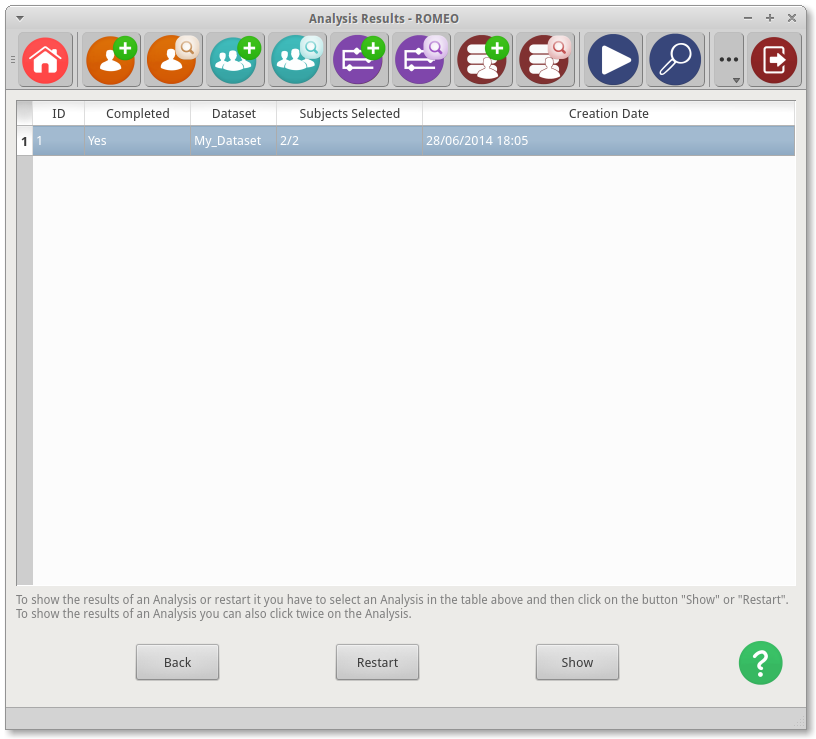
\includegraphics[scale=0.4]{./Images/AnalysisList}
\caption{\textit{Results visualization window}}
\label{visualizeresults}
\end{center}
\end{figure}
\pagebreak
To visualize the results of the executed analysis, follow these instructions:
\begin{itemize}
\item From the results visualization window, select the analysis of interest, from the list present in the left panel of the window;
\item Select the \textit{Show} button. Romeo will load the fig.\ref{detailedresults} window;
\item Navigate the file system in the left panel of the window to choose which results to visualize.
\end{itemize}
\begin{figure}[!h]
\begin{center}
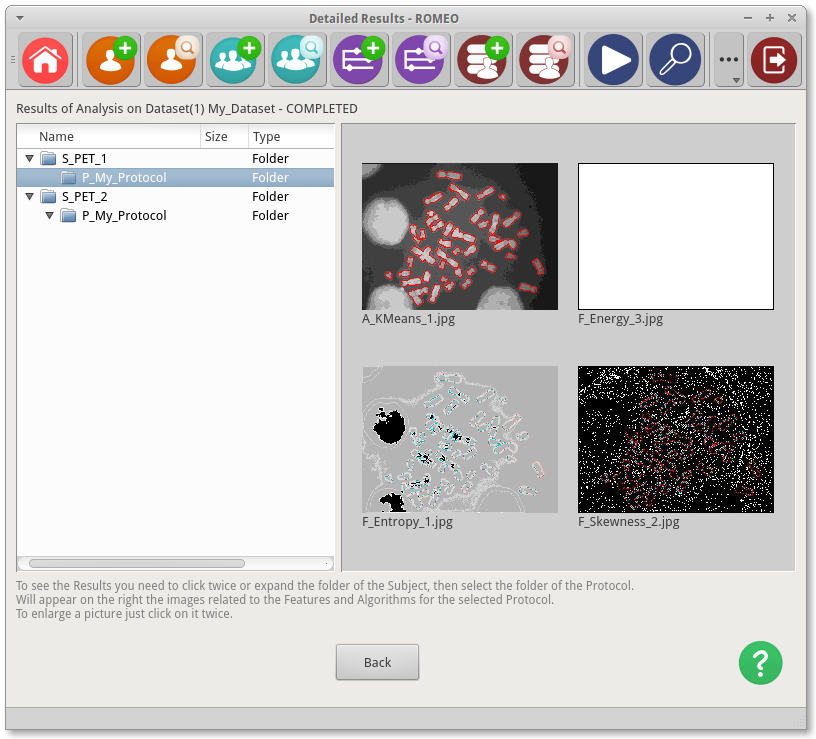
\includegraphics[scale=0.4]{./Images/ShowResults}
\caption{\textit{Detailed results visualization window}}
\label{detailedresults}
\end{center}
\end{figure}